\documentclass{article}
\usepackage[utf8]{inputenc}
\title{XinFOAM}
\usepackage{enumitem}
\usepackage[left=2.5cm,right=2.5cm,top=3cm,bottom=3cm]{geometry}
\usepackage{natbib}
\usepackage{graphicx}
\usepackage{xcolor}
\usepackage[colorlinks = true,
            linkcolor = blue,
            urlcolor  = blue,
            citecolor = blue,
            anchorcolor = blue]{hyperref}

\usepackage{pdflscape}
\usepackage{array}
\usepackage{makecell}
\renewcommand\theadalign{bc}
\renewcommand\theadfont{\bfseries}
\renewcommand\theadgape{\Gape[4pt]}
\renewcommand\cellgape{\Gape[4pt]}
\usepackage{geometry}
\usepackage{graphicx}
\usepackage{subcaption}
\captionsetup{justification=raggedright,singlelinecheck=false}

\begin{document}

\maketitle

\section{Numerical}
OpenFOAM applications are designed for use with unstructured meshes, offering up to second oder accuracy, predominately using collocated variable arrangements. Most focus on the Finite Volume Method, for which the conservative form of the general scalar transport equation for the property $\phi$ takes the form:

\begin{equation}
\underbrace{\frac{\partial}{\partial t} (\rho\phi)}_{\mathrm{unsteady}} + \underbrace{\nabla \cdot (\rho \phi \textbf{u})}_{\mathrm{convection}} = \underbrace{\nabla \cdot (\Gamma \nabla \phi)}_{\mathrm{diffusion}} + \underbrace{S_{\phi}}_{\mathrm{source}}
\label{eq:transport equation}
\end{equation}


\begin{table}[hbp!]
\begin{tabular}{l l}
	unsteady: &   time dependent\\
	convection & velocity dependent\\
	diffusion & viscosity dependent \\
	source & heat, force...
\end{tabular}
\end{table}
The finite volume method requires the integration over a 3D-control volume, such that:
\begin{equation}
\int_V \frac{\partial}{\partial t} {(\rho \phi)} dV + \int_V \nabla \cdot \left(\rho \phi \textbf{u} \right) dV = \int_V \nabla \cdot \left(\Gamma \nabla \phi \right) dV + \int_V S_\phi dV 
\label{eq:intergal transport equation}
\end{equation}
or in a more compact way:

\begin{equation}
\textit{\textbf{A}}\textbf{x} = \textbf{b}
\end{equation}
where
\begin{table}[hbp!]
\begin{tabular}{l l}
	A: &   coefficient matrix\\
	x & vector of unknows dependent\\
	b & source vector
\end{tabular}
\end{table}

The discretisation process employs user selected schemes to build the A matrix and b vector, described in the following sections. Choice of schemes are set in the \textit{fvSchemes} dictionary.

OpenFOAM includes a wide range of solution and scheme controls, specified via dictionary files in the case system sub-directory. These are described by:

Numerical schemes: The treatment of each term in the system of equations is specified in the fvSchemes dictionary. This enables fine-grain control of e.g. temporal, gradient, divergence and interpolation schemes.

Linear equation solvers Solution methods: Case solution parameters are specified in the fvSolution dictionary. These include choice of linear equation solver per field variable, algorithm controls e.g. number of inner and outer iterations and under-relaxation.

Finite volume options: Additional run-time selectable physical modelling and general finite terms are prescribed in the fvOptions dictionary, targeting e.g. acoustics, heat transfer, momentum sources, multi-region coupling, linearised sources/sinks and many more.

\subsection{Schemes}

\subsection{Temporal schemes}

OpenFOAM includes a variety of schemes to integrate fields with respect to time:

Time schemes

Time schemes define how a property is integrated as a function of time, i.e.
\begin{equation}
\frac{\partial}{\partial t}(\phi)
\end{equation}
Depending on the choice of schemes, field values at previous time steps are required, represented in the following as $\phi^0$ and $\phi^{00}$ for the old and older time levels. 

Usage 

Time schemes properties are input in the \textit{fvSchemes} file under the \textit{ddtSchemes} sub-directory using the syntax:

\begin{verbatim}
ddtSchemes
{
    default         none;
    ddt(Q)          <time scheme>;
}
\end{verbatim}
 
Available time schemes include
\begin{itemize}
\item Backward time scheme
\begin{equation}
\frac{\partial}{\partial t}(\phi) = \frac{1}{\Delta t}(\frac{3}{1}\phi - 2\phi^0 + \frac{1}{2} \phi^{00})
\end{equation}
Using implicit, second order accuracy, transient, boundedness not guaranteed, conditionally stable. 

Usage 

\begin{verbatim}
ddtSchemes
{
    default         backward;
    ddt(phi)        backward;
}
\end{verbatim}

\item Crank-Nicolson time scheme
Second order, Transient, Bounded, when using uniform time steps the schemes equate to: 
\begin{equation}
\frac{\partial}{\partial t} = \frac{\phi - \phi^{00}}{2\Delta t}
\end{equation}

Usage

The schemes is specified using: 

\begin{verbatim}
ddtSchemes
{
    default         CrankNicolson <coeff>
    ddt(phi)        CrankNicolson <coeff>;
}
\end{verbatim}

The coefficient provides a blending between Euler and Crank-Nicolson schemes:

0: Euler
1: Crank-Nicolson
A value of 0.9 is a good compromise between accuracy and robustness

\item Euler implicit time scheme

Implicit, First order, Transient 
\begin{equation}
\frac{\partial}{\partial t} = \frac{\phi - \phi^0}{\Delta t}
\end{equation}

Usage

\begin{verbatim}
ddtSchemes
{
    default         Euler;
    ddt(phi)        Euler;
}
\end{verbatim}


\item Local Euler implicit/explicit time scheme
First order
Pseudo transient, designed for steady cases
Spatially varying, cell-based time scale set by specific Local Time Stepping (LTS) solvers

Usage

\begin{verbatim}
ddtSchemes
{
    default         localEuler;
    ddt(phi)        localEuler;
}
\end{verbatim}

\item Steady state time scheme
Steady state, set temporal derivative contributions to zero, 
\begin{equation}
\frac{\partial}{\partial t} = 0
\end{equation}
\end{itemize}

\subsection{Spatial schemes}

At their core, spatial schemes rely heavily on \textit{interpolation schemes} to transform cell-bases qualities to cell faces, in combination with \textbf{Gauss Theorem} to convert volume integrals to surface integrals.

\begin{itemize}
\item Gradient Schemes
\item Divergence schemes
\item Laplacian schemes
\item Surface-normal gradient schemes
\end{itemize}

\subsection{Wall distance calculation method}

Distance to the nearest wall is required, e.g. for a number of turbulence models. Several calculation methods are available:
\begin{itemize}
\item Mesh-wave wall distance
\item Poisson wall distance 
\end{itemize}

\subsection{Solutions}

After using different schemes to build the equation systems. The next step is to chose a technic to solve the linear equations, the matrix sytem. 
\begin{equation}
x = A^{-1}b
\end{equation}
where the inverse of the diagonal matrix is simply:
\begin{equation}
A^{-1} = \frac{1}{dia(A)}
\end{equation}
This is available as the diagonalSolver. More tyically the matrix cannot be inverted easily and the system is solved using iterative methods, as discribed in the following sections. 

\subsection{Solvers}

\begin{itemize}
\item Smooth solvers
\item Conjugate gradient solvers
\item Multigrid solvers
\end{itemize}

\subsection{Solver control}
\begin{itemize}
\item Under relaxation
\item Residuals
\item Case termination
\end{itemize}

Common usage
minIter: minimum number of solver iterations
maxIter: maximum number of solver iterations
nSweeps: number of solver iterations between checks for solver convergence
Implementation details
Matrix structure
Matrix coefficients are stored in upper-triangular order

neighbour cell index always higher than owner cell index across a face
when looping over cell faces, the face index increases with increasing cell index
for the 1-D case, if cell index 0 is at the boundary, this equates to a monotonic increase in cell numbers, i.e. defines a continuous sweep across the 1-D region
used in Gauss-Seidel method


\section{boundary condition}

Boundary conditions are extremely important. Indeed, they cause the most common errors.
OpenFOAM uses similar set-up as other solvers.
\begin{itemize}
    \item At the inlet (flow inlet) to the computational domain total pressure and total temperature are set. The rest of variables are reconstructed.
    \item At the outlet the static pressure is set.
    \item At the rigid walls velocity is set to zero.
    \item Multiple Reference Frame (MRF) is used for rotational components.
    \item For steady-state computations the initial conditions have no influence to the results.
    \item For steady-state computations the initial conditions just help to make the case run.
\end{itemize}

The main variables to be set are following:

p: static pressure p

U: velocity vector U

T: static temperature

k: turbulent kinetic energy k

$\omega$: specific turbulence dissipation 

$\epsilon$ specific turbulence dissipation

The initial and boundary conditions for all variables are set in files located in directories named by numbers. Typically directory 0 is recommended to start a simulation from. 

Initial conditions are set in parameter internalField putting the values into the cell centres. 

At boundaries, initial conditions are set individually by parameter value.

Following table shows recommended model of boundary conditions for computed variables:


\begin{landscape}
\begin{table}[h!]
    \centering
\begin{tabular}{cccccc}

\hline
boundaty type & p & U  & T & k & $\omega$ / $\epsilon$\\  
\hline
   	 	STATOR:	 \\
   	 	\hline
inlet &	totalPressure &	\makecell{pressureDirected\\InletVelocity} &	totalTemperature &	\makecell{turbulentIntensity\\KineticEnergyInlet} &	fixedValue   \\
volute\_wall &	zeroGradient &	fixexValue &	\makecell{compressible::\\turbulentTemperature\\CoupledBaffeMixed} &	\makecell{compressible::\\kqRWallFunction}	 & \makecell{compressible::\\omegaWallFunction}\\
ring* &	mixingPlane &	inletOutlet &	inletOutlet &	 inletOutlet &	inletOutlet\\
\hline	 	 	 	  
 	 	ROTOR	 	 	 \\
 	 	\hline
outlet &	fixedMeanValue &	inletOutlet &	inletOutlet	 & inletOutlet &	inletOutlet \\
outlet wall &	zeroGradient &	fixedValue	 & \makecell{compressible::\\turbulentTemperature\\CoupledBaffeMixed}	 & \makecell{compressible::\\kqRWallFunction} &	\makecell{compressible::\\omegaWallFunction} \\
wheel wall &	zeroGradient &	fixexValue &	zeroGradient	 & \makecell{compressible::\\kqRWallFunction} & 	\makecell{compressible::\\omegaWallFunction} \\
ring* &	zeroGradient &	mixingPlaneVelocity &	mixingPlane &	mixingPlane &	mixingPlane \\
\hline	 	 	 	 	  
 	 	SOLID:	 	 	 \\
 	 	\hline
rotor inner wall &	x &	x &	\makecell{compressible::\\turbulentTemperature\\CoupledBaffeMixed} &	x &	x \\
stator inner wall &	x &	x &	\makecell{compressible::\\turbulentTemperature\\CoupledBaffeMixed} &	x &	x \\
outer wall &	x &	x &	zeroGradient &	x &	x \\

  \hline

\end{tabular}
    \caption{Boundary condition recommondation$^*$}
    \label{tab:CFD-support recomm}
\end{table}

$^*$: taken from: 
\url{https://www.cfdsupport.com/Turbomachinery-CFD-manual/node283.html\#13201}
\end{landscape}






The shortcuts from the above table have following meaning:
\begin{itemize}
    \item tP - totalPressure constant, e.g. 250 000 Pa, gamma = 1.2853 [-] is specific heat ratio
    \item pDIV - pressureDirectedInletVelocity, velocity is computed from difference between total and static pressure, inletDirection is velocity vector to be specified
    \item tT - totalTemperature, constant, e.g. 1050 K, gamma= 1.2853 [-] is specific heat ratio
    \item tIKEI - turbulentIntensityKineticEnergyInlet, intensity = 0.02, corresponds to turbulence intensity 2%
    \item fV - fixedValue, e.g. velocity at the wall (0 0 0), or omega at inlet
    \item fMV - fixedMeanValue, is the same as fixed value, e.g. for pressure, but certain freedom is allowed to keep the variable average equal to meanValue
    \item zG - zeroGradient, the flux of the variable is zero in direction perpendicular to the surface
    \item TWF - compressible::turbulentTemperatureCoupledBaffleMixed special boundary condition for temperature enabling heat transfer from other regions
    \item kWF - compressible::kqRWallFunction is a standard wall function for k for compressible flow
    \item oWF - compressible::omegaWallFunction is a standard wall function for omega for compressible flow
    \item mPV - mixingPlaneVelocity, averaged velocity is mapped from neighbour patch
    \item mP - mixingPlane, averaged variable is mapped from neighbour patch
    \item iO - inletOutlet is by default zeroGradient, but changes to fixedValue when velocity vector direction points inside the computational domain (backward flow)
\end{itemize}


Another recommended boundary conditions for each vairable (depending on the selected turbulence model) at each boundary type. Note the variations for Wall BCs for a High Reynolds model(y+ 30-100), and a Low Reynolds model(y+ 1).


\newgeometry{left=1cm,right=1cm,top=1cm,bottom=1cm}
\begin{landscape}


\begin{table}[h!]
    \centering
\begin{tabular}{ccccccc}
\hline
  & inlet & outlet  & farfield & stationary walls & moving walls & rotating walls\\  
\hline
p &	\textbf{zeroGradient} &	\textbf{fixedValue 0 }&	\textbf{outletInlet 0} &	\textbf{zeroGradient} &	\textbf{zeroGradient}  & \textbf{zeroGradient}\\

U &	\makecell{\textbf{surfaceNormalFV} \\ negative value for \\ entry velocity}  &	\makecell{\textbf{zeroGradient} \\ \textbf{inletOutlet}}  & \makecell{\textbf{inletOutlet} \\ free stream velocity} & \makecell{\textbf{fixedValue 0}}	 & \makecell{\textbf{fixedValue}\\ velocity of the wall}  & \makecell{\textbf{rotatingWallVelocity} \\rotational \\velocity of the wall}\\

k &	\makecell{\textbf{fixedValue} \\ k = $(3/2)*(UI)^2$\\U:free stream velocity \\ I: Turbulent intensity} &	\makecell{\textbf{zeroGradient} \\ \textbf{inletOutlet}} & \makecell{ \textbf{inletOutlet} \\ k = $(3/2)*(UI)^2$\\U:free stream velocity \\ I: Turbulent intensity} & \makecell{\textbf{kqRWallFunction}\\(for y+ 30 to 100)\\\textbf{fixedValue 0} \\ (for y+ 1)}  & \makecell{\textbf{kqRWallFunction}\\(for y+ 30 to 100)\\\textbf{fixedValue 0} \\ (for y+ 1)} & \makecell{\textbf{kqRWallFunction}\\(for y+ 30 to 100)\\\textbf{fixedValue 0} \\ (for y+ 1)} \\

epsilon &\makecell{\textbf{fixedValue} \\ $\epsilon=0.09*k*\omega$} &	\makecell{\textbf{zeroGradient} \\ \textbf{inletOutlet}} &\makecell{ \textbf{inletOutlet} \\  $\epsilon=0.09*k*\omega$}	 & \makecell{\textbf{epsilonWallFunction} \\ (for y+ 30 to 100) \\ fixedValue $10^{-12}$ \\ (for y+ 1) }&	\makecell{\textbf{epsilonWallFunction} \\ (for y+ 30 to 100) \\ fixedValue $10^{-12}$ \\ (for y+ 1) } & \makecell{\textbf{epsilonWallFunction} \\ (for y+ 30 to 100) \\ fixedValue $10^{-12}$ \\ (for y+ 1) } \\

omega & 	\makecell{\textbf{fixedValue} \\ $\omega = \rho*\frac{k}{\mu}*(\frac{\mu_t}{\mu})^{-1}$\\ $\rho$:Density \\ k:Turbulence \\ kinetic energy \\ $\mu$: viscosity \\ $\mu_t$:turbulent viscosity} &	\makecell{\textbf{zeroGradient} \\ \textbf{inletOutlet}}	 & \makecell{\textbf{inletOutlet} \\ $\omega = \rho*\frac{k}{\mu}*(\frac{\mu_t}{\mu})^{-1}$\\ $\rho$:Density \\ k:Turbulence kinetic energy \\ $\mu$: viscosity \\ $\mu_t$:turbulent viscosity}	 &  \textbf{omegaWallFunction} &	\textbf{omegaWallFunction}  & \textbf{omegaWallFunction}\\

nutTilda &	\makecell{\textbf{fixedValue} \\ nuTilda = $\sqrt{3/2}*U*I*L$ \\ U:free stream velocity \\ I:turbulent intensity \\L:length scale} &	\makecell{\textbf{zeroGradient} \\ \textbf{inletOutlet}} & \makecell{\textbf{inletOutlet} \\ nuTilda = $\sqrt{3/2}*U*I*L$ \\ U:free stream velocity \\ I:turbulent intensity \\L:length scale}	 & \makecell{\textbf{zeroGradient} \\ (for y+ 30 to 100) \\ \textbf{fixexValue 0} \\ (for y+ 1)} & 	\makecell{\textbf{zeroGradient} \\ (for y+ 30 to 100) \\ \textbf{fixexValue 0} \\ (for y+ 1)} & \makecell{\textbf{zeroGradient} \\ (for y+ 30 to 100) \\ \textbf{fixexValue 0} \\ (for y+ 1)}  \\

nut & \textbf{calculated} &	\textbf{calculated} & \textbf{calculated}  &	\makecell{\textbf{nutkWallFunction} \\ (for y+ 30 to 100) \\ \textbf{nutUSpalding}\\\textbf{WallFunction} \\ (for y+ 1)} & \makecell{\textbf{nutkWallFunction} \\ (for y+ 30 to 100) \\ \textbf{nutUSpalding}\\\textbf{WallFunction} \\ (for y+ 1)} & \makecell{\textbf{nutkWallFunction} \\ (for y+ 30 to 100) \\ \textbf{nutUSpalding}\\\textbf{WallFunction} \\ (for y+ 1)}\\
\end{tabular}
    \caption{Boundary condition recommondation$^*$}
    \label{tab:ANSA recomm}
\end{table}
$^*$: taken from: 
ANSA for CFD Brief User's Guide. v19.1.2

\end{landscape}
\restoregeometry

\begin{landscape}
\begin{table}[h!]
    \centering
\begin{tabular}{cccccccccccc}

\hline
solver & transient & compressible  & turbulence & \makecell{heat\\transfer} & buoyancy & combustion & \makecell{multi\\phase} & particles& dynamicMesh & \makecell{multi\\region} & fvOptions\\  
\hline
boundaryFoam \\
\hline
buoyantPimpleFoam & $\surd$ & $\surd$ & $\surd$ & $\surd$ & $\surd$ & & & & & & $\surd$  \\
\hline
buoyantSImpleFoam & & & $\surd$ & $\surd$ & $\surd$ & $\surd$ & & & & & $\surd$ \\
\hline
chemFoam & $\surd$ & & & $\surd$ & & $\surd$ & & & & & \\
\hline
chtMultiRegionFoam & $\surd$ & $\surd$ & $\surd$ & $\surd$ & $\surd$ & & & & & $\surd$ & $\surd$ \\
\hline
coldEngineFoam & $\surd$ & $\surd$ & $\surd$ & $\surd$ & & $\surd$ & & & $\surd$ & & $\surd$ \\
\hline
engineFoam & $\surd$ & $\surd$ & $\surd$ & $\surd$ & & $\surd$ & & & $\surd$ & & $\surd$ \\
\hline
fireFoam & $\surd$ & $\surd$ & $\surd$ & $\surd$ & $\surd$ & $\surd$ & & & & $\surd$ & $\surd$ \\
\hline
icoFoam & $\surd$ & & & & & & & & & & \\
\hline
interFoam & $\surd$ & & $\surd$ & & & & $\surd$ & & $\surd$ & & $\surd$ \\
\hline
laplacianFoam & $\surd$ & & & & & & & & & & $\surd$ \\
\hline
pimpleFoam & $\surd$ & & $\surd$ & & & & & & $\surd$ & & $\surd$ \\
\hline
pisoFoam & $\surd$ & & $\surd$ & & & & & & & & $\surd$ \\
\hline
potensialFoam \\
\hline
reactingFoam & $\surd$ & $\surd$ & $\surd$ & $\surd$ & & $\surd$ & & & & & $\surd$ \\
\hline
reactingParcelFoam & $\surd$ & $\surd$ & $\surd$ & $\surd$ & $\surd$ & $\surd$ & & $\surd$ & & & $\surd$ \\
\hline
rhoCentralFoam & $\surd$ & $\surd$ & $\surd$ & $\surd$ & & & & & &  & \\
\hline
rhoPimpleFoam & $\surd$ & $\surd$ & $\surd$ & $\surd$ & & & & & $\surd$ & & $\surd$ \\
\hline
rhoSimpleFoam & & $\surd$ & $\surd$ & $\surd$ & & & & & & &  $\surd$\\
\hline
scalarTransportFoam & $\surd$ & & & & & & & & & & \\
\hline
simpleFoam & & & & & & & & &  & & $\surd$ \\	
\hline
spratFoam & $\surd$ & $\surd$ & $\surd$ & $\surd$ & $\surd$ & $\surd$& & $\surd$ & & & $\surd$ \\
\hline
XiFoam & $\surd$ & $\surd$ & $\surd$ & $\surd$ & & $\surd$ & & & & & $\surd$\\
\hline
\end{tabular}
    \caption{application solver capability matrix$^*$}
    \label{tab:solver compatibility}
\end{table}
$^*$: taken from: 
\url{https://www.openfoam.com/documentation/guides/latest/doc/openfoam-guide-applications-solvers.html#sec-applications-solvers-capability-matrix}

\end{landscape}



\section{Conclusion}
``I always thought something was fundamentally wrong with the universe'' \citep{adams1995hitchhiker}
 
\begin{figure}[h!]
\centering
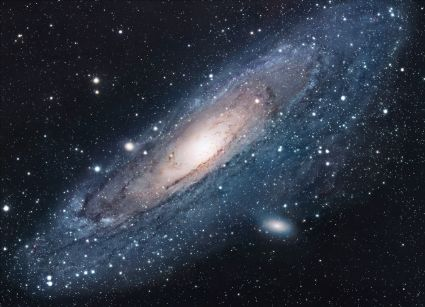
\includegraphics[width=0.8\textwidth,natwidth=610,natheight=642]{universe.jpg}
\caption{The Universe}
\label{fig:universe}
\end{figure}

\appendix
\section{Gauss Theorem}
\begin{equation}
\int_V(\nabla \cdot u) dV = 
\end{equation}

\bibliographystyle{plain}
\bibliography{references}
\end{document}
